
\section{Introduction}
\sectionmark{Introduction}
\label{sec:introtask} 



As neuroscience seeks to characterize the principles governing brain function, task-based functional magnetic resonance imaging (fMRI) has emerged as an important tool for investigating the relationship between cognitive processes and neural activity. Carefully controlled experimental paradigms enable the identification of functionally specialized brain regions in relatively short scanning sessions, based on the hypothesis that the blood-oxygen-level-dependent (BOLD) response in task-relevant regions will be stronger and temporally more structured than in task-irrelevant regions \citep{poldrackRegionInterestAnalysis2007, saxeDivideConquerDefense2006, gloverDeconvolutionImpulseResponse1999}.

This underlying assumption facilitates the delineation of functionally distinct cortical regions. Although the spatial location of these regions can vary substantially across individuals, their localization is generally stable within a given individual \citep{duboisBuildingScienceIndividual2016, fernandezIntrasubjectReproducibilityPresurgical2003, yoo2005long, cohenStabilityRepeatabilityExpression1999, grattonFunctionalBrainNetworks2018a}. One straightforward strategy to enhance the reliability and specificity of functional activation patterns is to increase the number of task runs, thereby improving sensitivity \citep{zandbeltSubjectVariationBOLDfMRI2008}.

A canonical example is face perception, for which a specialized region in the human ventral temporal cortex, the fusiform face area (FFA), shows markedly increased responses to faces relative to other object categories \citep{kanwisherFusiformFaceArea1997}. Although the precise anatomical locus of the FFA within the fusiform gyrus is subject dependent, its functional selectivity for faces is highly robust across individuals \citep{bermanEvaluatingFunctionalLocalizers2010}.

\citet{stiglianiTemporalProcessingCapacity2015} developed a block-design visual localizer paradigm to characterize the selectivity of cortical responses to distinct stimulus categories (e.g., faces, bodies, places, objects, and orthographic characters). In this paradigm, the fusiform face area (FFA) is identified using the contrast faces $>$ all. In the present work, we implement an adapted language-focused version of this paradigm that additionally incorporates word stimuli, thereby enabling the assessment of both perceptual and lexical sensitivity, alongside the original face and body conditions \citep{lerma-usabiagaConvergingEvidenceFunctional2018,OHBM2026Tiger}.

Given the increasing demand for high–spatial resolution acquisitions to detect task-sensitive regions, thermal noise reduction has become essential for improving signal quality in low–signal-to-noise ratio (SNR) regimes. In single-echo acquisitions, NORDIC denoising has been shown to substantially increase task-evoked response estimates within regions of interest for both visual and auditory paradigms \citep{vizioli2021lowering, dowdle2023evaluating, faesEvaluatingEffectDenoising2024}. \citet{dowdle2023evaluating} demonstrated that, for a visual task, NORDIC increased task-related $t$ statistics and the number of responsive voxels, and additionally improved the goodness-of-fit between time series predicted by a general linear model (given a design matrix) and the observed fMRI data.

Multi-echo acquisition has been shown to enhance fMRI sensitivity and therefore represents a promising approach for improving BOLD sensitivity at higher spatial resolution \citep{kundu2012differentiating}. However, as high-spatial-resolution imaging becomes increasingly common, an optimal framework for exploiting the combined advantages of multi-echo acquisitions and thermal noise suppression has yet to be fully articulated for task-specific studies. 

In this work, we investigate the most effective thermal denoising strategy for multi-echo fMRI in the context of task-based research, comparing several approaches (i.e., non-denoised “vanilla” data, MP-PCA, NORDIC, and temporal MP-PCA). We assess the impact of these denoising methods on signal stability by quantifying improvements in time-series prediction based solely on design information. Subsequently, we evaluate their influence on functional sensitivity by examining our ability to detect the fusiform face area (FFA) and by characterizing the magnitude of the task-related response, as estimated from model fits across runs during the response modeling stage.






\section{Method}
\sectionmark{MethodsT}




\subsection{Image Acquisition Parameters}
\subsectionmark{Image Acquisition Parameters}
\label{ImageParametersT}

    Task-related fMRI runs were acquired on a 3T MAGNETOM PrismaFit scanner (Siemens Healthineers) equipped with a 64-channel head coil at the Basque Center on Cognition, Brain, and Language. The primary objective of the dataset was to characterize the influence of thermal denoising on multi-echo acquisitions within a functional localizer fMRI paradigm. All runs employed simultaneous multi-slice (SMS) echo-planar imaging with in-plane GRAPPA acceleration. Single-band reference (SBRef) images were acquired for each echo time (TE). For all runs, both magnitude and phase images were reconstructed. In addition, the last three noise-only volumes of each run were retained, as these data are required for the NORDIC thermal noise reduction procedure. Finally, T1-weighted MP2RAGE and T2-weighted turbo spin-echo images were acquired at 1 mm isotropic resolution.

\textbf{1.5 mm dataset (high resolution, single subject)} A healthy male participant was scanned with a three-echo fMRI sequence during four sessions of ten runs ( 5 min per run) at 1.5 mm isotropic resolution (TR = 2 s, TEs = 16/46.92/77.84 ms, SMS = 4, partial Fourier (PF) = 6/8, GRAPPA = 2). The principal aim of this dataset is to examine the effect of denoising in a functional localizer task at the highest spatial resolution that is practically attainable at 3T, a regime in which thermal noise is the predominant determinant of the signal-to-noise ratio (SNR).

\textbf{Stimuli} MRI data were acquired using a block-design localizer paradigm \citep{lerma-usabiagaConvergingEvidenceFunctional2018, OHBM2026Tiger}, modeled after the protocol described in \citet{stiglianiTemporalProcessingCapacity2015}. Each run comprised 51 blocks of 6 s duration, presented in randomized order (42 active blocks and 9 baseline blocks). Individual stimuli were presented for 400 ms with a 100 ms inter-stimulus interval (ISI).  The stimulus set encompassed five domains (e.g., faces, bodies, LEX, PER, words). Participants performed a one-back repetition detection task to monitor and quantify attentional engagement via response accuracy and were not considered for attention unless accuracy was equal or above $70\%$ leading to a total of 22 analyzable runs. The attentional threshold is held high to maximize the signal coming from the design. 

\begin{figure}
    \centering
    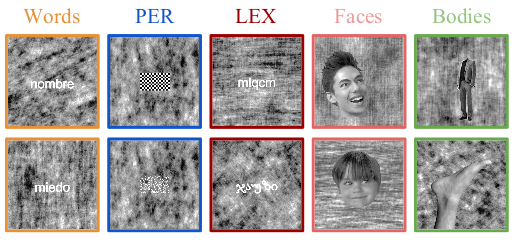
\includegraphics[width=6cm]{images/task.png}
    \caption[Functional-localizer stimuli domain]{Functional-localizer stimuli domain. For each experimental run, 48 randomized active block encompassed one of these stimuli: \textit{words} (high \& low frequency), \textit{PER} (scrambled words \& checker boards), \textit{LEX} (consonants strings \& false fonts), \textit{faces} (adults \& children faces), \textit{bodies} (limbs \& bodies with obscured heads). Image reproduced from \citet{OHBM2026Tiger}}
    \label{fig:placeholder}
\end{figure}





\textbf{Thermal denoising} The dataset was independently denoised using different algorithms prior to minimal preprocessing: undenoised (vanilla), MP-PCA, NORDIC, NORDIC applied to spatially concatenated echoes (HYDRA), and tensor MP-PCA (TMPPCA).


\textbf{fMRI preprocessing} Multi-echo (ME) fMRI data were minimally preprocessed using AFNI. The preprocessing pipeline included discarding the initial 10 volumes to ensure steady-state magnetization, realigning the first echo to the single-band reference (SBRef) image, and applying the resulting transformation parameters to all remaining echoes. For the high-resolution dataset, all runs were additionally aligned to the SBRef of the first run using a local Pearson correlation cost function (\texttt{align\_epi\_anat.py}, \texttt{3dAllineate}). A T2\textbf{*}-weighted optimal linear combination of the echoes was subsequently computed using TEDANA (multi-echo optimal combination, ME-OC). To rigorously assess the robustness of the thermal denoising approaches, no motion censoring was applied, with the understanding that this choice may degrade signal quality and thereby render time-series predictions noisier.
 

 \textbf{Region of interest (ROI) creation} The anatomical image was segmented using FreeSurfer (version 7.4.0) with the \texttt{recon-all} pipeline \citep{fischl2004automatically}. The resulting segmentations were subsequently transformed into AFNI volumetric space using the \texttt{@SUMA\_Make\_Spec\_FS} utility. A custom ROI mask was then generated with AFNI’s \texttt{3dcalc}, incorporating the bilateral cortical gray-matter ribbons as well as subcortical structures. 

From the SUMA output, a skull-stripped anatomical volume was rigid-body aligned to the single-band reference (sbref) image of the first echo. The alignment was estimated using local Pearson correlation as the cost function. The resulting transformation matrix was then applied to the ROI mask to register it from anatomical space into functional space. 


\section{Analysis}

    

\textbf{Event-based general linear model (GLM):} For each denoising strategy, a general linear model (GLM), as implemented in the Nilearn, and Scikit with Python 3.11 , was fitted to gray-matter–masked time series after standardizing each voxel’s signal across time ( $\widehat{S}(t) = \frac{S(t) - \bar{S}}{\bar{S}} $ ), thereby ensuring comparability across runs.

An event-related design was specified in which event time courses were convolved with the canonical hemodynamic response function (HRF) provided by Nilearn (Glover HRF model). Event onsets and durations were defined according to the run-specific design matrix. In addition, the first four orders of nuisance regressors were included in the model. All regressors were entered simultaneously into a first-level GLM, which was estimated independently for each run. Motion parameters were deliberately excluded as regressors to avoid capturing variance that is not predictable from the experimental design and thus cannot contribute to cross-run generalization.

To obtain task-specific parameter estimates (beta coefficients), linear contrasts were specified to isolate the contribution of each experimental condition independently.

\textbf{Task-localizer contrast sensitivity:}  
We applied general linear model (GLM) fitting to the functional localizer data to assess whether thermal denoising enhances sensitivity for detecting spatially specific BOLD responses. For this analysis, we focused on the contrast (Faces $>$ all) to identify face-selective regions, such as the fusiform face area, given that their selectivity is robustly characterized using functional localizers \citep{bermanEvaluatingFunctionalLocalizers2010}. The analysis was conducted on the first run of our dataset, while systematically varying the number of runs included in the GLM estimation (e.g., 1, 2, 3, …) to quantify how sensitivity metrics change across denoising strategies as a function of the amount of data used for model fitting.
% GLM predict
\begin{figure}[htbp]
    \centering
    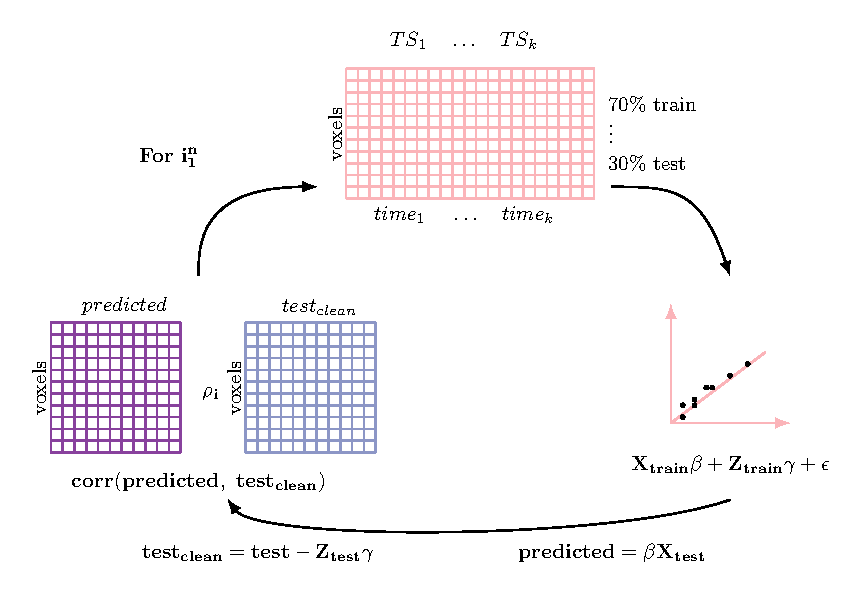
\includegraphics[width=11cm]{images/glmpredict.pdf}
    \caption[Task-related Time-series Prediction after linear model fitting (GLM predict)]{Task-related time series prediction following linear model fitting (GLM-based prediction). First, all available runs are randomly assigned to either a training set ($70\%$) or a test set ($30\%$). Within each set, runs are temporally concatenated after converting the signal to percent signal change. 

Second, a general linear model (GLM) is fitted to the training data using the task design matrix \(X_{\text{train}}\) and four low-order polynomial regressors modeling temporal drift as nuisance covariates \(Z_{\text{train}}\gamma\). The predicted time series for the test data are then obtained by multiplying the task design matrix for the test set, \(X_{\text{test}}\), by the estimated parameter vector \(\hat{\beta}\). Subsequently, the concatenated test time series are denoised by regressing out their drift nuisance regressors \(Z_{\text{test}}\gamma\). 

Goodness-of-fit is quantified voxel-wise as the Pearson correlation between the predicted time series and the drift-cleaned observed time series. This entire procedure is repeated for \(i\) iterations.}
    \label{fig:GLMreliability}
\end{figure}


\textbf{Task-related time series prediction (GLM predict):} A cross-validation permutation procedure was employed to evaluate the accuracy of task-specific parameter estimates following GLM fitting for each denoising strategy (see Fig.~\ref{fig:GLMreliability} for an illustration of the full procedure) \citep{princeImprovingAccuracySingletrial2022,dowdle2023evaluating}. This analysis was designed to assess how thermal denoising strategies influence the capacity of task-specific parameters to generalize to activation patterns in independent runs, under the assumption that increased time-series sensitivity via noise reduction should improve cross-run validation. The random seed was held constant across strategies and permutations to ensure comparable train–test splits.

For each permutation, $70\%$ of the runs were randomly selected for GLM fitting (training) and the remaining $30\%$ were reserved for testing. For the test datasets, the first four orders of nuisance regressors were projected out so that the residual variance could be attributed to, and thus predicted from, the experimental design alone.

After GLM fitting, event-specific beta estimates were multiplied by the design matrix of the test runs to generate predicted time series for each voxel. Prediction accuracy was quantified by computing the coefficient of determination, $r^{2}$, between the predicted and observed time series for each voxel. Finally, we reported the mean per-voxel $r^{2}$ across permutations to enable comparison between denoising strategies.


\section{Results}


\subsection{GLM predict}
\begin{figure}[htbp]
\centering \colorbox{black}{
    \centering
    \begin{tabular}{>{\centering\arraybackslash}m{1cm}>{\centering\arraybackslash}m{5cm}>{\centering\arraybackslash}m{5cm}}
       & \textcolor{white}{\textbf{VANILLA}} & \textcolor{white}{\textbf{MPPCA}} \\
    &    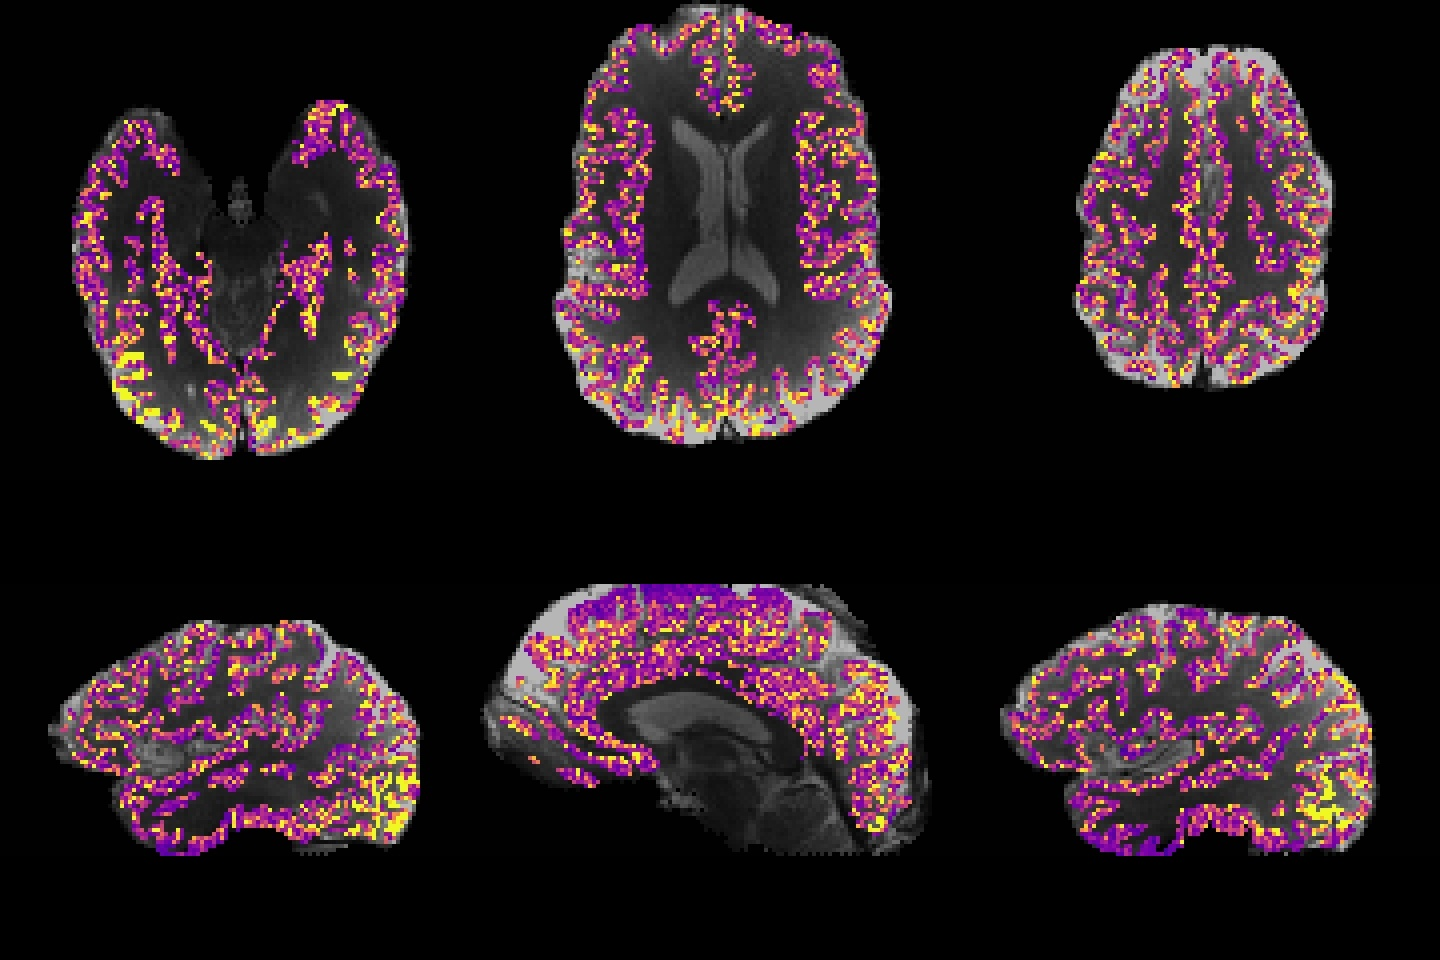
\includegraphics[width=5cm]{images/vanilla_task_real_mean_r2_all.jpg} &
        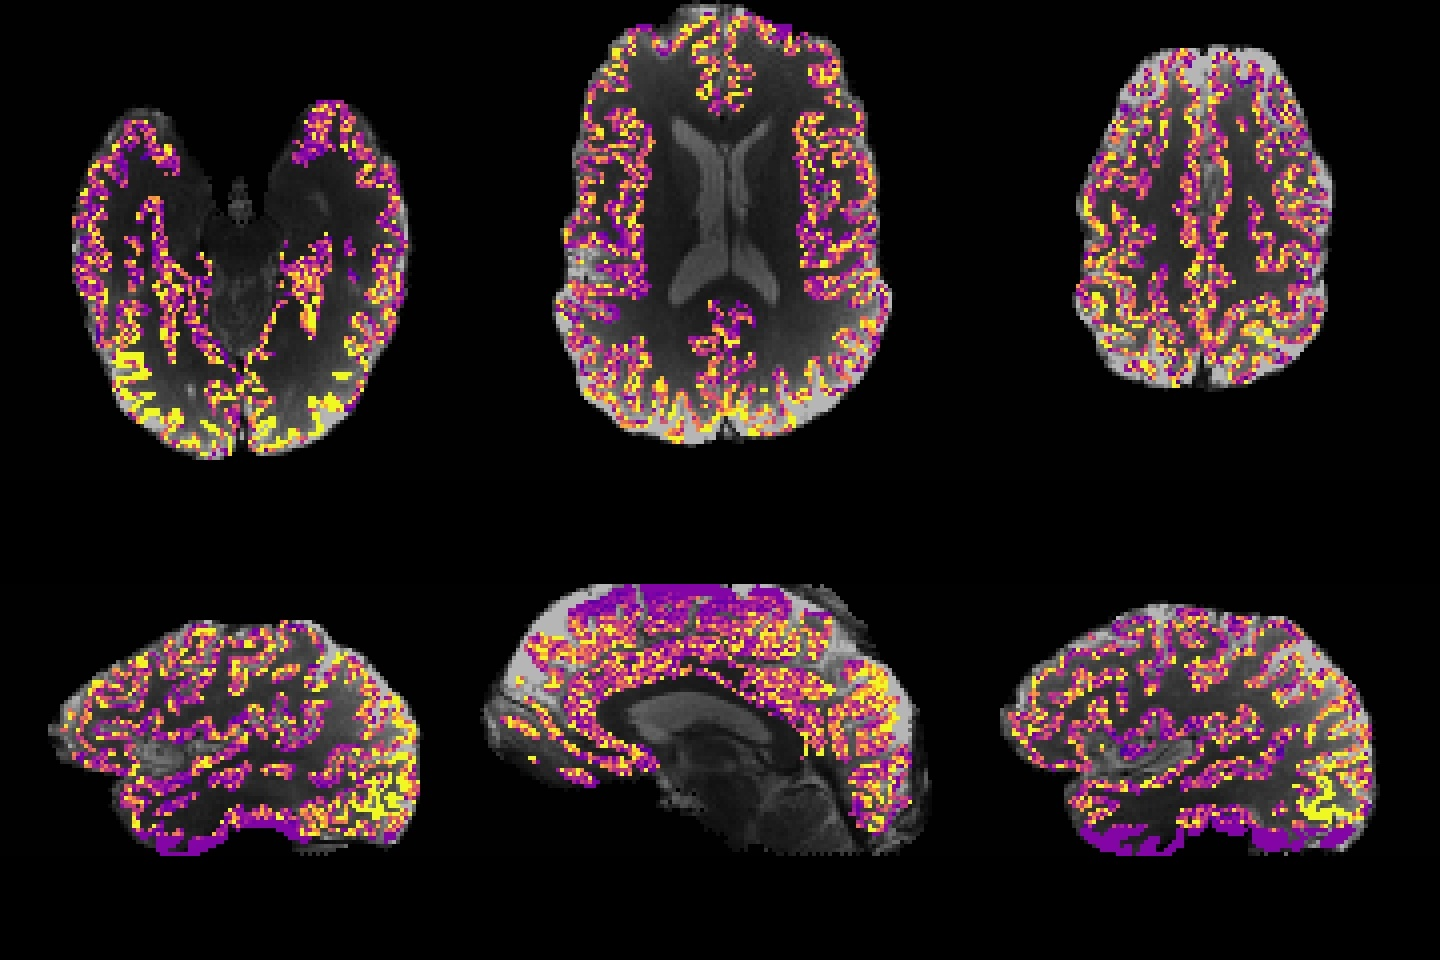
\includegraphics[width=5cm]{images/mppca_task_real_mean_r2_all.jpg}\\
      &   \textcolor{white}{\textbf{NORDIC}}& \textcolor{white}{\textbf{HYDRA}}\\
        
\includegraphics[width=.5cm]{images/Plasmaglm.png}&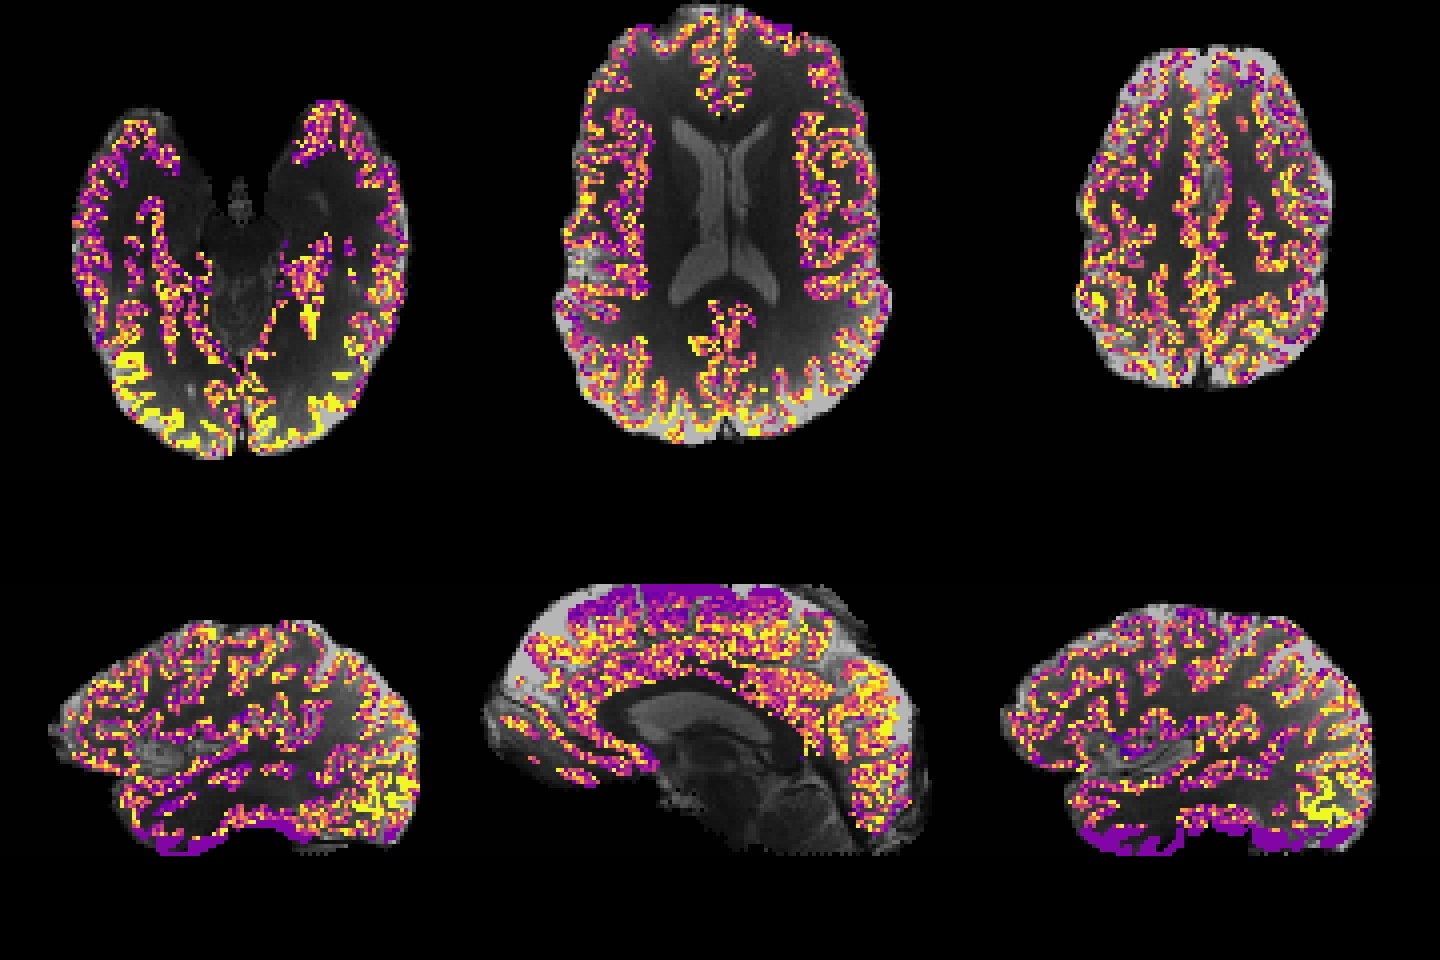
\includegraphics[width=5cm]{images/nordic_task_real_mean_r2_all.jpg} &
        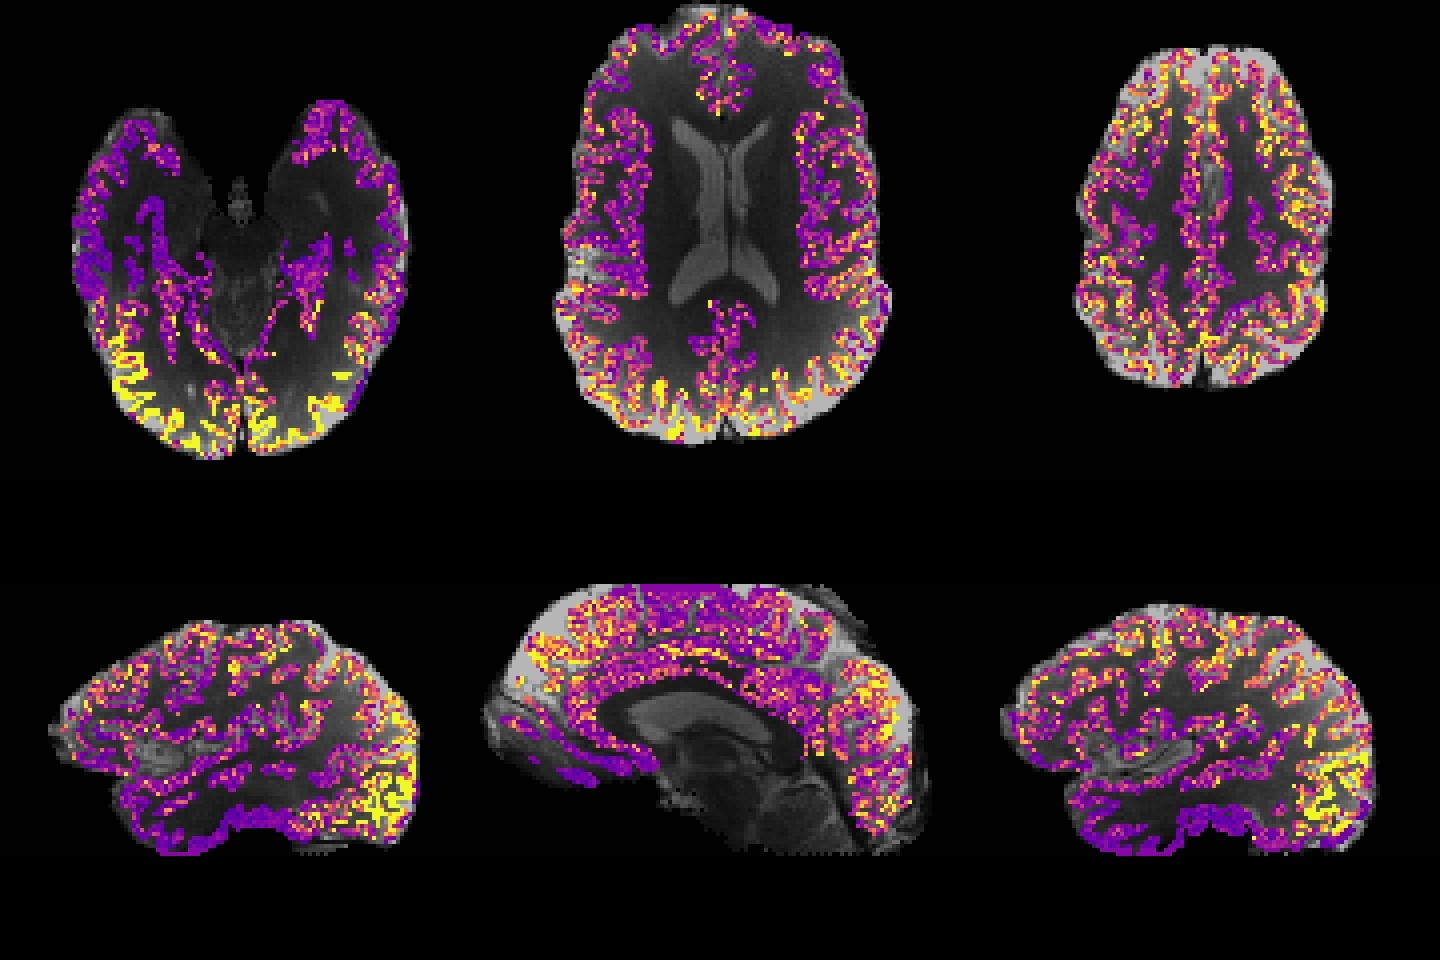
\includegraphics[width=5cm]{images/hydra_task_real_mean_r2_all.jpg}\\
          &       \multicolumn{2}{c}{\textcolor{white}{\textbf{TMPPCA}}}\\
      &  \multicolumn{2}{c}{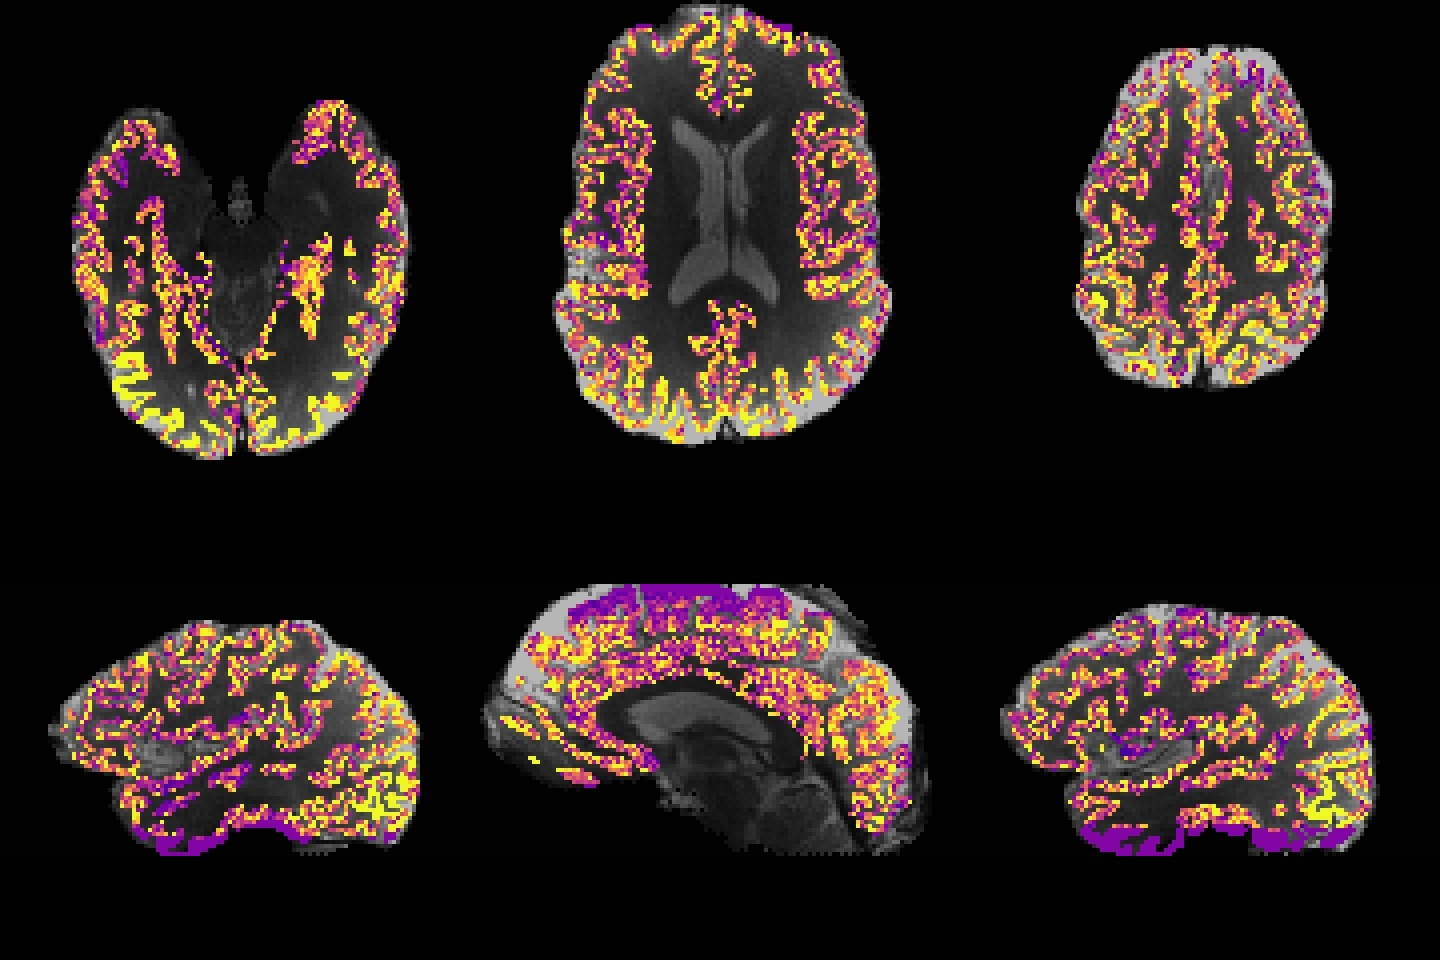
\includegraphics[width=5cm]{images/tmppca_task_real_mean_r2_all.jpg}} \\
    \end{tabular}
    }
    \caption[Average goodness-of-fit ($r^2$) between minimally preprocessed time series and voxel-wise predictions]{Average goodness-of-fit ($r^2$) between minimally preprocessed time series and voxel-wise predictions from GLM fitting (100 iterations). As thermal denoising reduces random variance and stabilizes the signal, the linear predictability of the time series—and consequently the $r^2$—is expected to increase. MPPCA, NORDIC, and TMPPCA all yield higher $r^2$ saturation, with TMPPCA achieving the highest scores overall.} 
    \label{fig:glmPredictr2}  
\end{figure}

\begin{figure}[htbp]
    \centering
    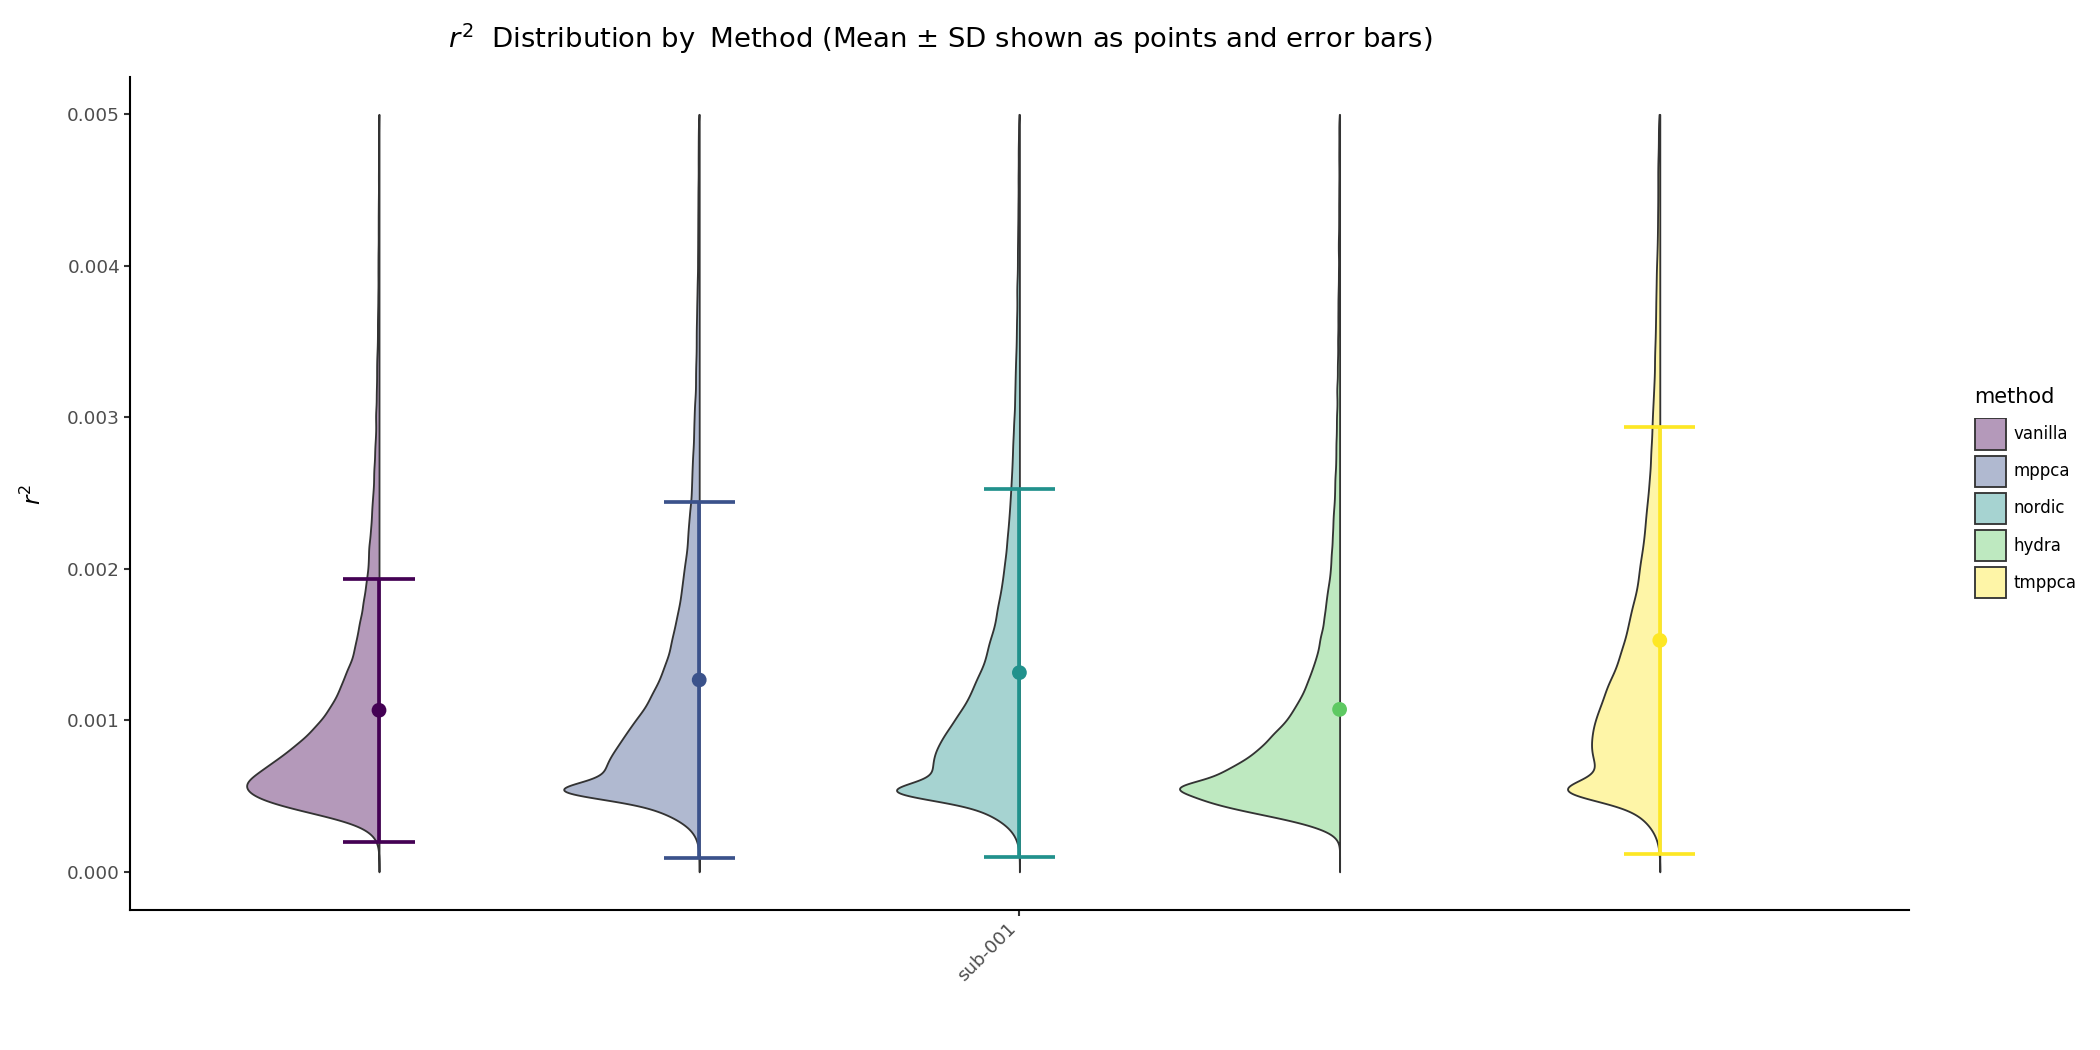
\includegraphics[width=12cm]{images/halfviolin_glm_across_subjects_masked.png}
    \caption[Distribution of goodnes-of-fit score, $r^2$ after time-series prediction across 100 iterations per method]{Distribution of goodness-of-fit scores ($r^2$) from time-series prediction across 100 iterations per method. Thermal denoising consistently increases $r^2$, as reflected by heavier tails skewed toward higher values. By reducing variance, denoising shifts the distribution away from unimodality toward bimodality, presumably with gains predominantly affecting voxels likely reflecting task-induced activity. TMPPCA yields the largest improvement, followed by NORDIC and MPPCA. Notably, HYDRA underperforms relative to the vanilla condition, consistent with resting-state findings at this voxel resolution (1.5 mm isotropic).}
    \label{fig:glmdist}
\end{figure}


    
The objective of this analysis was to evaluate the efficacy of thermal denoising in preserving task-related signal by quantifying the discrepancy between predicted time series, derived from the corresponding design matrices, and empirically observed time series. The analysis was performed over 100 iterations and was restricted to runs with the highest behavioral accuracy (22 runs in total).

Mean $r^2$ maps for each denoising strategy demonstrate clear differences in model goodness-of-fit (Fig.~\ref{fig:glmPredictr2}). Using VANILLA as the reference condition, a substantial improvement in $r^2$ is observed following thermal denoising, with overall performance following the pattern HYDRA $>$ VANILLA $>$ MPPCA $>$ NORDIC $>$ TMPPCA. In agreement with the resting-state analysis at 1.5 mm isotropic resolution, HYDRA outperforms NORDIC. These results provide strong evidence that increasing spatial redundancy in NORDIC denoising does not improve, and may in fact attenuate, the task-relevant signal.

For the VANILLA dataset, the highest $r^2$ scores were localized to task-relevant cortical regions (e.g., visual cortex), as expected given that these areas most strongly reflect design-induced signal changes. For denoising strategies that yielded increased $r^2$ values, the improvement in goodness-of-fit was not restricted to regions with high task-evoked responses but extended across the entire gray matter. This pattern indicates enhanced robustness of the underlying signal, leading to more reliable beta estimates and reduced random signal fluctuations.

The distribution of $r^2$ scores (Fig.~\ref{fig:glmdist}) further supports the beneficial impact of thermal denoising, as evidenced by heavier distribution tails skewed towards higher values. In addition to the overall increase in $r^2$, the distribution shifts from unimodal to bimodal, presumably reflecting a clearer separation between task-sensitive and non–task-sensitive voxels. This analysis suggests that thermal denoising increases the proportion of variance in the time series that can be attributed to the experimental design alone. We anticipate that a more fine-grained analysis restricted to strongly task-responsive regions would yield even more pronounced improvements.

This analysis primarily assesses the overall generalizability of model fitting, approximating scenarios encountered in standard first-level fMRI analyses. It is important to note that, because this analysis evaluates prediction of the full time series rather than task-specific segments alone, residual confounds such as motion-related artifacts may still degrade signal quality. To more directly characterize the gain in sensitivity conferred by thermal denoising, we therefore conducted an additional analysis focusing on the task-localizer contrast sensitivity for faces.






\subsection{Task-localizer contrast sensitivity}


The objective of this analysis was to assess changes in sensitivity in a functional localizer task following the application of thermal denoising procedures. We examined the effect on sensitivity when fitting the GLM using one, two, or three runs. Under the assumption that only signal components of no interest are removed, we would expect an increase in $t$-values and its spread after denoising. In addition, incorporating a greater number of runs into the GLM fit should, in principle, further increase $t$-values.

The $t$-maps for each denoising strategy across different numbers of runs per GLM fit show clear differences in sensitivity, manifested as increased saturation as a function of the number of runs and its interaction with the denoising method (Fig.~\ref{fig:localizer}). Consistent with the resting-state analysis, we find that HYDRA underperforms relative to NORDIC, which further supports the notion that the spatial redundancy introduced by spatial echo concatenation adversely affects $tSNR$ and sensitivity in high-resolution acquisitions.

Notably, the $t$-maps for the VANILLA condition exhibit more values close to zero both within and outside the FFA. In contrast, for the denoised strategies, the increase in $t$-values predominantly occurs in regions expected to be task-sensitive. This pattern indicates that variance attributable to non–task-related effects is reduced, which in turn leads to higher $t$-statistics for the task-relevant effects. This patter is more evident in TMPPCA, where higher saturation happens in all three comparisons when compared to the other strategies.








\begin{figure}[htbp]
\centering \colorbox{black}{
    \centering
    \begin{tabular}{>{\centering\arraybackslash}m{.7cm}>{\centering\arraybackslash}m{3cm}>{\centering\arraybackslash}m{3cm}>{\centering\arraybackslash}m{3cm}>{\centering\arraybackslash}m{.7cm}}
    
       & \textcolor{white}{\textbf{1 run}} & \textcolor{white}{\textbf{2 runs}} &\textcolor{white}{\textbf{3 runs}} \\
   \rotatebox[origin=l]{90}{\textcolor{white}{VANILLA}}
  &    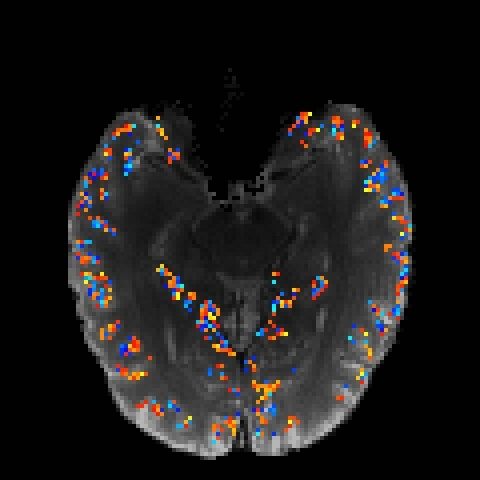
\includegraphics[width=3cm]{images/sub-001_ses-1_task-fLoc_run-1_OC_part-mag_bold_vanilla_localizer1_all} &     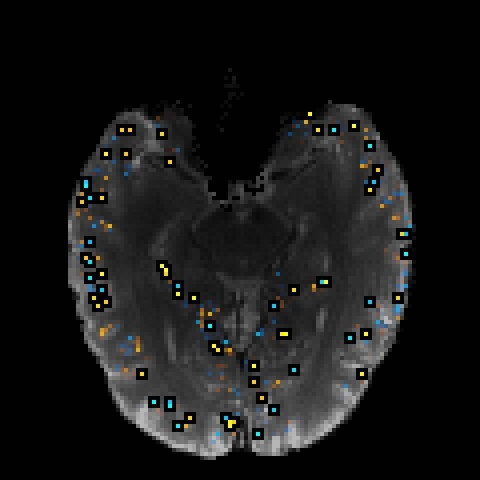
\includegraphics[width=3cm]{images/sub-001_ses-1_task-fLoc_run-1_OC_part-mag_bold_vanilla_localizer2_all} &
      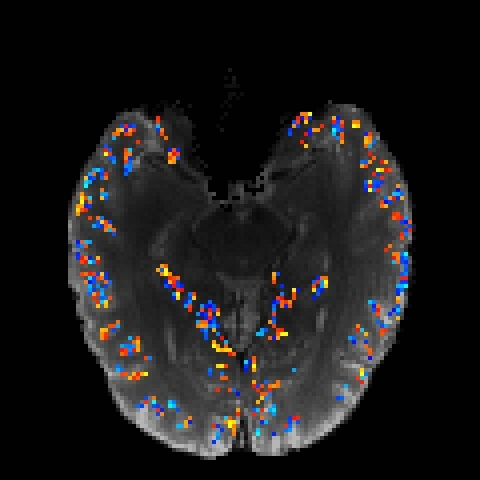
\includegraphics[width=3cm]{images/sub-001_ses-1_task-fLoc_run-1_OC_part-mag_bold_vanilla_localizer3_all}& \\
   \rotatebox[origin=l]{90}{\textcolor{white}{MPPCA}}
  &    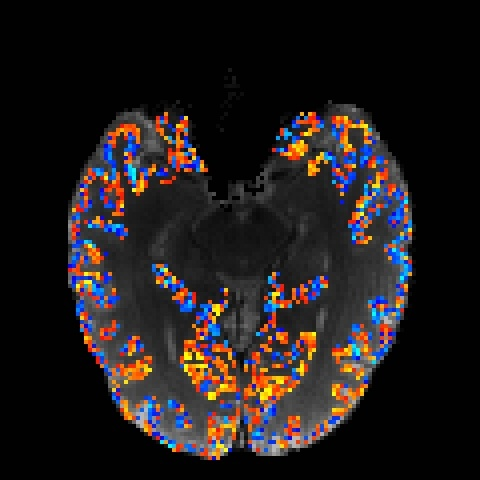
\includegraphics[width=3cm]{images/sub-001_ses-1_task-fLoc_run-1_OC_part-mag_bold_mppca_localizer1_all} &     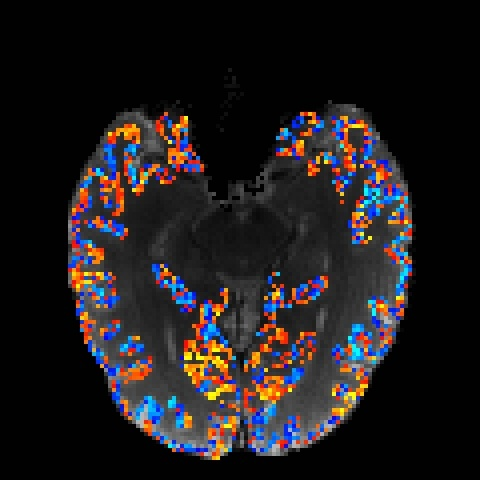
\includegraphics[width=3cm]{images/sub-001_ses-1_task-fLoc_run-1_OC_part-mag_bold_mppca_localizer2_all} &
      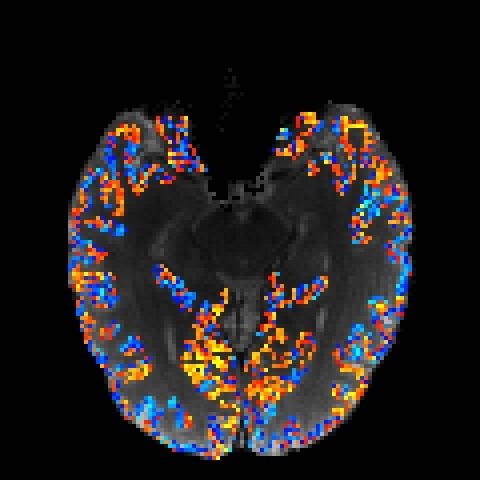
\includegraphics[width=3cm]{images/sub-001_ses-1_task-fLoc_run-1_OC_part-mag_bold_mppca_localizer3_all}&\\
   \rotatebox[origin=l]{90}{\textcolor{white}{NORDIC}}
  &    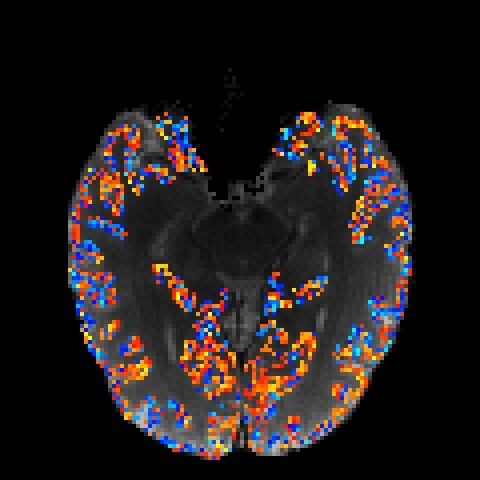
\includegraphics[width=3cm]{images/sub-001_ses-1_task-fLoc_run-1_OC_part-mag_bold_nordic_localizer1_all} &     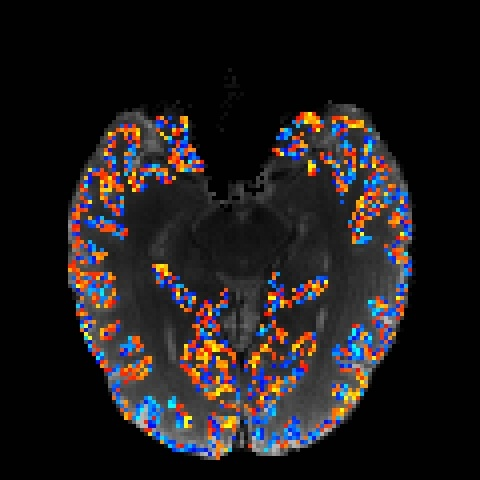
\includegraphics[width=3cm]{images/sub-001_ses-1_task-fLoc_run-1_OC_part-mag_bold_nordic_localizer2_all} &
      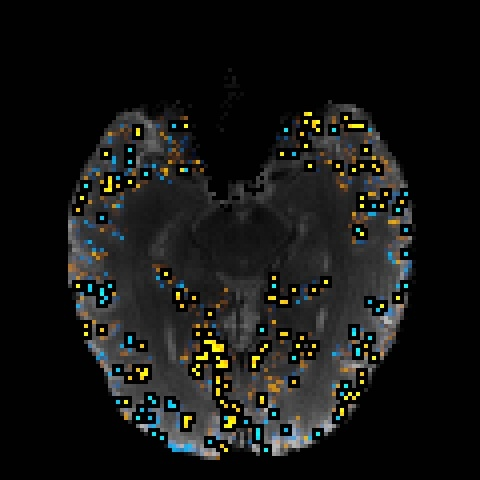
\includegraphics[width=3cm]{images/sub-001_ses-1_task-fLoc_run-1_OC_part-mag_bold_nordic_localizer3_all}&\textcolor{white}{\textbf{$t$}} 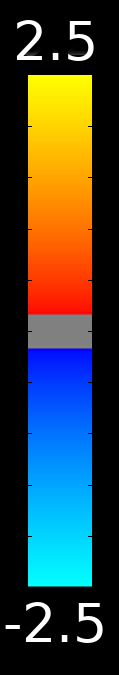
\includegraphics[width=.5cm]{images/yellow2cyan_t.png}\\
   \rotatebox[origin=l]{90}{\textcolor{white}{HYDRA}}
  &    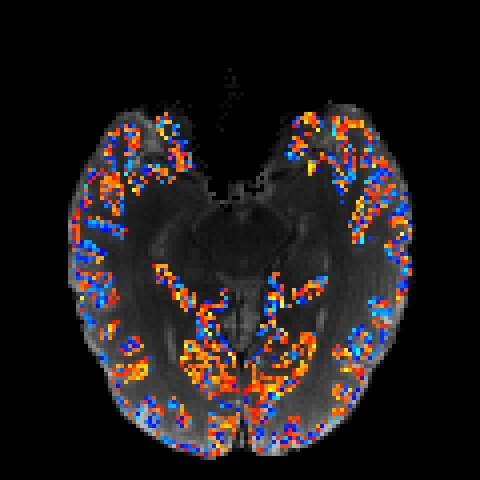
\includegraphics[width=3cm]{images/sub-001_ses-1_task-fLoc_run-1_OC_part-mag_bold_hydra_localizer1_all} &     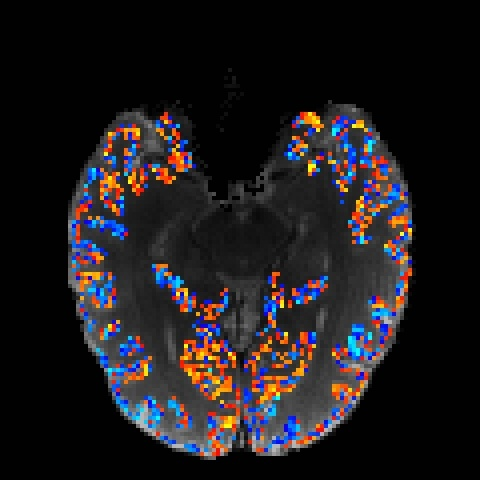
\includegraphics[width=3cm]{images/sub-001_ses-1_task-fLoc_run-1_OC_part-mag_bold_hydra_localizer2_all} &
      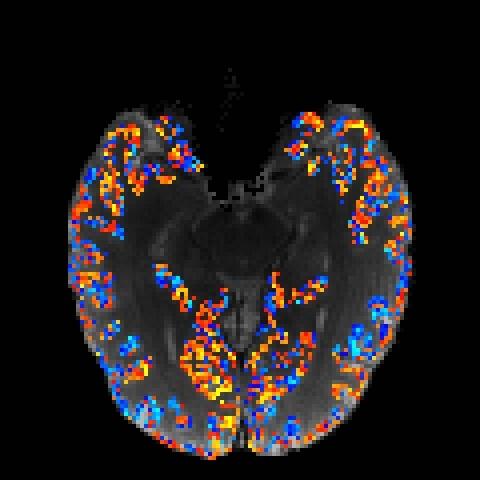
\includegraphics[width=3cm]{images/sub-001_ses-1_task-fLoc_run-1_OC_part-mag_bold_hydra_localizer3_all}&\\
   \rotatebox[origin=l]{90}{\textcolor{white}{TMPPCA}}
  &    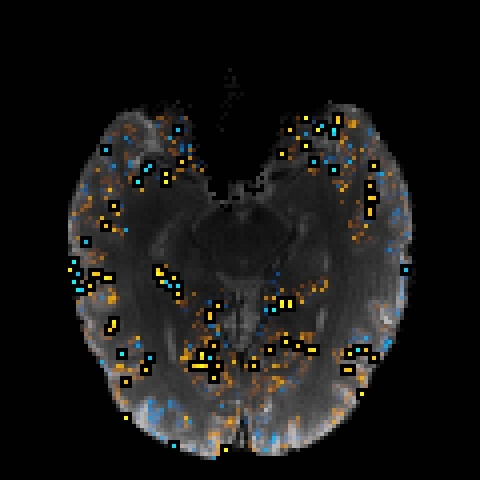
\includegraphics[width=3cm]{images/sub-001_ses-1_task-fLoc_run-1_OC_part-mag_bold_tmppca_localizer1_all} &     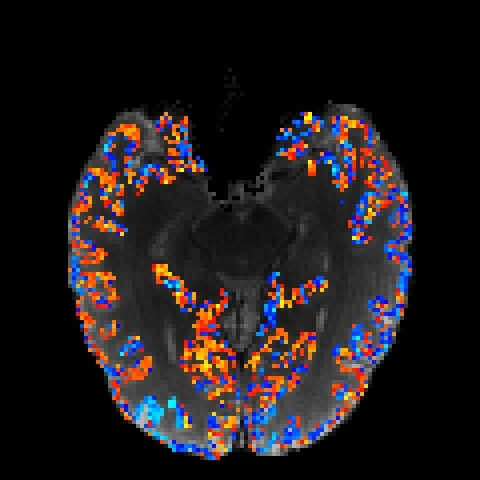
\includegraphics[width=3cm]{images/sub-001_ses-1_task-fLoc_run-1_OC_part-mag_bold_tmppca_localizer2_all} &
      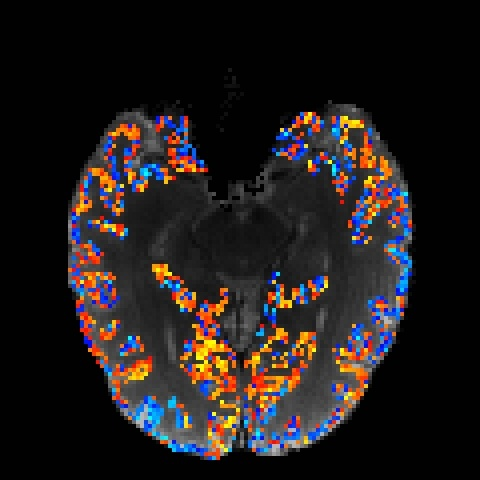
\includegraphics[width=3cm]{images/sub-001_ses-1_task-fLoc_run-1_OC_part-mag_bold_tmppca_localizer3_all}&\\
    \end{tabular}
    }
    \caption[Functional localizer t-statistic maps (faces > all other conditions) and their modulation as a function of the number of runs]{Functional localizer t-statistic maps (faces > all other conditions) and their modulation as a function of the number of runs used to train the GLM (one, two, or three runs) are presented. Maps are thresholded and saturated at t = 2.5. First, we confirm the sensitivity of both the task and all denoising strategies, as evidenced by increased activation in the Fusiform Face Area (FFA). Second, we observe that thermal denoising increases the extent and saturation of higher t-values relative to the undenoised (vanilla) data. Among the evaluated methods, TMPPCA exerts the strongest effect on t-map saturation, indicating a substantial gain in sensitivity attributable to the removal of signal components not related to the task of interest.  }
    \label{fig:localizer}
\end{figure} 

\section{Discussion}


Our objective is to determine the optimal denoising strategy, within a task-based paradigm, for applying thermal noise suppression to high‑resolution multi‑echo acquisitions. In previous work, we demonstrated that TMPPCA outperforms NORDIC, HYDRA, and MPPCA on signal quality metrics in resting‑state acquisitions (see Chap. \ref{chap:denoising}). Here, we extend this evaluation to task‑based data, assessing the extent to which thermal denoising enhances sensitivity to task‑evoked brain activity, thereby improving the utility of functional imaging for neuroscience \citep{poldrackRegionInterestAnalysis2007}. Consistent with prior findings, thermal denoising improves signal quality \citep{zhu2022denoise,comby2023denoising}.

Because thermal denoising is expected to remove variance unrelated to the experimental manipulation, it should yield data that are more amenable to linear modeling for effect detection. We evaluated this using GLM prediction analyses, which quantify the amount of signal that can be predicted from the design matrix alone, as well as the accuracy with which test time series can be predicted from their corresponding design \citep{princeImprovingAccuracySingletrial2022}. In agreement with reports from single‑echo acquisitions, NORDIC improves the goodness of fit between predicted and observed time series, outperforming MPPCA and HYDRA \citep{dowdle2023evaluating}. However, we found that TMPPCA, applied in the tensorial domain, yields the best overall performance \citep{olesenTensorDenoisingMultidimensional2023}.

TMPPCA produced a higher saturation of $r^2$ values compared with the other approaches. Moreover, thermal denoising induced a transformation in the distribution of voxelwise $r^2$ values from unimodal to bimodal. Given that not all gray‑matter voxels are expected to be task sensitive, reliability scores should preferentially increase in task‑selective regions. This selective enhancement is consistent with the emergence of a bimodal distribution, and this shift was most pronounced for TMPPCA.

To further quantify the beneficial effect of denoising on task‑selective voxels, we assessed the reliability of identifying the fusiform face area (FFA) at the single‑subject level after using one, two, or three runs for model fitting \citep{kanwisherFusiformFaceArea1997}. As anticipated, thermal denoising increased sensitivity to task‑specific activations by enhancing both the magnitude and extent of responsive voxels. However, this increased sensitivity also raises the possibility that some activations may reflect statistical artifacts introduced by denoising procedures \citep{kay2022riskL,fernandesMPPCADenoisingFMRI2023a}.

Across all evaluations, TMPPCA, followed by NORDIC, provided the most favorable results, producing higher and more spatially localized $t$‑statistics. Notably, we observed superior performance when fitting a GLM to a single run of TMPPCA‑denoised data relative to undenoised data. This pattern held across all denoising strategies, whereby a single run of denoised time series outperformed the VANILLA (undenosed) condition.





\section{Conclusions}

    

We investigated the impact of thermal denoising on multi‑echo sensitivity to BOLD‑induced effects, thereby extending the scope of our findings to task‑based analyses.

With respect to signal sensitivity, we found that thermal denoising increases the proportion of variance explained by the task design alone. This indicates that the mere application of thermal denoising enhances sensitivity to task‑related signal changes driven by the BOLD response. Furthermore, we confirmed that TMPPCA yields the largest improvement in signal predictability. Although NORDIC also enhances predictability relative to VANILLa and MPPCA, its effect is less pronounced than that of TMPPCA.

In a more fine‑grained analysis of signal sensitivity, we observed that thermal denoising leads to an increase in both the magnitude and the number of statistically significant $t$‑values, thereby facilitating localization of the FFA. As expected, increasing the number of runs improved activation localization. Among the evaluated strategies, TMPPCA substantially improved localization of task‑related regions even with a single run, and this advantage became more pronounced with three runs. Consistent with previous reports, NORDIC provided the second‑largest improvement.

Our analyses demonstrate that, at high spatial resolution, thermal denoising is a feasible and effective strategy for enhancing task sensitivity. Moreover, our results consistently show that TMPPCA achieves the best overall performance, followed by NORDIC. 

 

